\documentclass[a4paper,11pt]{article}
\usepackage[a4paper,total={18cm, 24cm}]{geometry}
\usepackage[parfill]{parskip}
\usepackage[utf8]{inputenc}
\usepackage[T1]{fontenc}
\usepackage{fancyhdr}
\usepackage[ddmmyyyy]{datetime}
\usepackage{graphicx}
\usepackage{subcaption}

\pagestyle{fancy}
\fancyhf{}
\lhead{\today}
\chead{Deep Learning - Backpropagation}
\rhead{Jakub Rada}

\begin{document}
\section{Part 1: Tensor basics}
In this part of the assignment we go through some basics of pytorch \texttt{tensors} and computing gradients.
The code is provided in a file \texttt{tensor\_task.py}, this report contains answers to questions and drawings of computation graphs.

\paragraph{(2)} Draw the computation graph for the used expression.
\begin{figure}[ht]
    \centering
    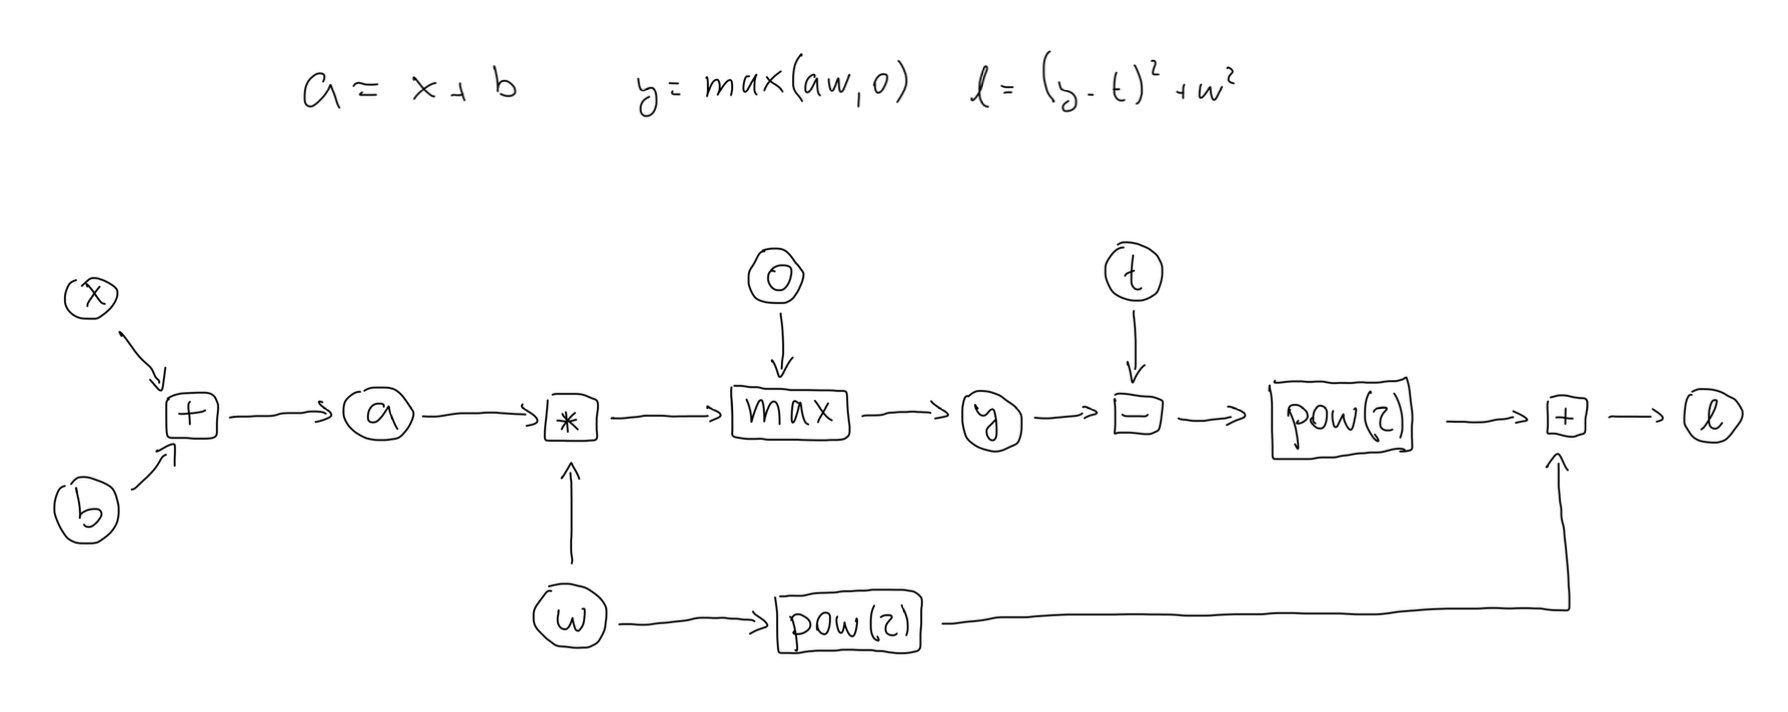
\includegraphics[width=0.8\textwidth]{./DAG.png}
\end{figure}

\texttt{graph\_fn} attributes are as follows:
\begin{table}[ht]
    \centering
    \begin{tabular}{r | l}
        variable & \texttt{graph\_fn}    \\
        y        & \texttt{MulBackward0} \\
        l        & \texttt{AddBackward0} \\
        a        & \texttt{None}         \\
    \end{tabular}
\end{table}

\paragraph{(3)} Derivative of $l$ w.r.t. $y$ is $6.0$.

\paragraph{(4)} Derivative of $l$ w.r.t. $w$ is $38.0$.

\paragraph{(5)} The new value of $w^{\prime} = w - 0.1\nabla_{w}l = -2.799999952316284$.
We need to access the \texttt{.data} attribute because if we added it to the whole tensor, PyTorch would save this update to the computation graph and future backgpropagation could depend also on this computation instead of just the forward pass.
This would lead to wrong results.

\paragraph{(6)} The gradient will be computed correctly, because references to the used tensors are stored in the computation graph, so the garbage collector will not remove them when leaving the scope of the function.
It will remove only the references bound to the variable names.
Also, the \texttt{del} is redundant because the variable references will be removed automatically when the program leaves the scope of the function.

The commented \texttt{y /= 2} causes an error because we try to modify an inner node of the computation graph after it was already used in the forward pass.
This would either lead to inconsistent values of the tensors in the graph or all computations following y in the graph would have to be recomputed again, which does not make sense.

\end{document}
